\section{Project}
\subsection{Adopted Databases}
According to concept presented in the previous chapter we can make the following considerations:
\begin{enumerate}
\item Because of the performance constraint, a fast backend is required. Moreover, since the aim is to spread the application worldwide, the database infrastructure should be easy to distribute.
\item \textbf{Pokémon} must store heterogeneous data like URLs, different kinds of bios, float arrays and so on.
\item \textbf{Users} are divided into normal users and admins. Although the second ones are few, a denormalized approach could be better to handle the fact that these two categories have very different attributes.
\item Rankings are real-time OLAP queries: they need fast aggregation strategies.
\item Favorite Pokémon, Friends, Posts and Answers together form a real Social Network.
\item A \textbf{Team}, in a normalized relational model, could be seen as a relationship table between Users and Pokémon. Anyway, a huge table with a lot of duplicated PokémonID is not scalable due to the requirements of this application. There is a need to find the best way to perform quickly both the retrieving of a \textbf{User}’s team and the ranking of the most used \textbf{Pokémon}, optimizing if possible memory consumption.
\end{enumerate}

The points 1 to 4 guided the choice of a \textbf{Document Database} for handling User and Pokémon data. The flexibility, denormalization and performance of this kind of the database make it the most appropriate one.\medspace \\

The point 5 is best handled by a \textbf{Graph DB}, optimized for networks and different kinds of relationships. Moreover, we realized that the best way to handle a team is to decompose it in a set of Graph Relationships (USER – OWNS $\rightarrow$ POKEMON).  Indeed, in this way queries mentioned at point 6 are very fast (just counting incoming/outcoming edges, see paragraph 3.3.1), and there are no useless, waste-memory repetitions of User IDs/Pokémon IDs. \\
Since each user can have only a team, team name and points are stored in the user collection.


\subsection{Document Database}
\subsubsection{Queries Handled}
\begin{itemize}
	\item Insert a \textbf{User} into the system at registration time
	\item Create a new \textbf{Pokémon} (admin only)
	\item Retrieve \textbf{User} information at login time
	\item Retrieve a \textbf{User} by username
	\item Retrieve \textbf{Pokémon} information using several filters
	\item Retrieve a \textbf{Pokémon} by name when trying to catch it
	\item Modify \textbf{User} settings (email, password, country)
	\item Update \textbf{Team}’s name
	\item Update \textbf{Team}’s points
	\item Update \textbf{Pokémon}’s catch rates 
	\item Remove a \textbf{User} (admin only)
	\item Remove a \textbf{Pokémon} (admin only)
	\item Analytics: ranking of best \textbf{Teams} in the world/each country/among friends
	\item Analytics: evolution on time of a \textbf{Pokémon} catch rate
	\item Analytics: evolution on time of number of logins per day/total \textbf{Users}/logins per day by country (admin only)
\end{itemize}
\subsubsection{Entities handled}
Document Database stores information about \textbf{Users} and \textbf{Pokèmons}. \medspace \\ 

In particular it remembers \textbf{User}’s anagraphics and login data, last login, remaining Pokéballs, team name and earned points; a Boolean field distinguish admin from normal users. Admins have no points nor team or Pokéballs.\\

In a separate collection are stored data about \textbf{Pokémon}: PokédexId (source: PokeAPI), characteristics, one or more types, bio, images URLs, current capture$\_$rate and its last 30 catch$\_$rates stored into an array of Floats.\\

The details of the collections are reported in the following paragraph.

\subsubsection{Collections structure}
\begin{figure}[H]
	\centering
	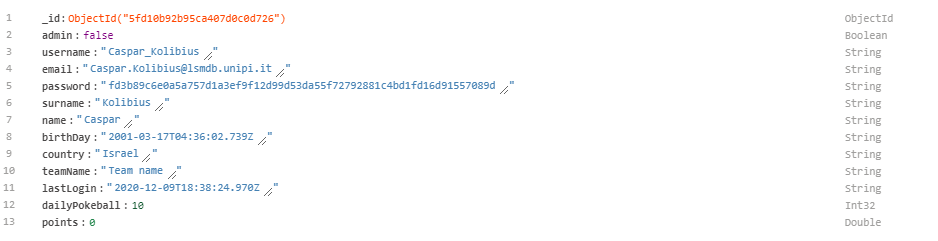
\includegraphics[width=\textwidth]{img/user_collection.png}
	\caption{User Collection}
\end{figure}
Relevant Attributes:
\begin{itemize}
	\item \textit{Admin}: \textbf{true} $\rightarrow$ admin, \textbf{false} $\rightarrow$ normal user
	\item \textit{Username}: unique mnemonic ID of the user
	\item \textit{Email}: must respect typical e-mail format
	\item \textit{Password}: encrypted version of the user-chosen password
	\item \textit{Last Login}: timestamp of the last time the user logged into the application
	\item \textit{dailyPokeball}: number of daily Pokéballs left. They are up to 10 per day
	\item \textit{points}: worth of his/her team
\end{itemize}

\begin{figure}[H]
	\centering
	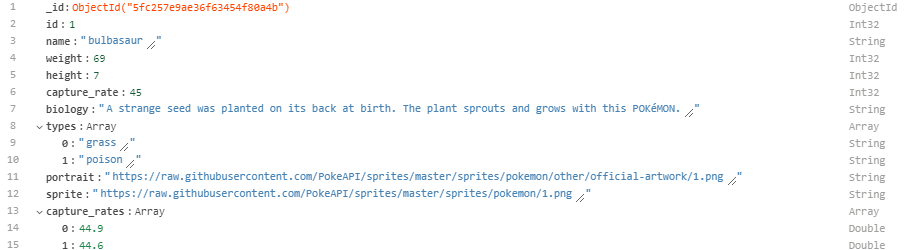
\includegraphics[width=\textwidth]{img/pokemon_collection.png}
	\caption{Pokèmon Collection}
\end{figure}
Relevant Attributes:
\begin{itemize}
	\item \textit{Id}: Pokédex ID (unique)
	\item \textit{Name}: unique mnemonic ID of the Pokémon
	\item \textit{Capture$\_$Rate}: current index of probability to catch the Pokémon
	\item \textit{Portrait/Sprite}: URLs of the graphical representations of this Pokémon
	\item \textit{Capture$\_$Rates}: array of the last 30 values of the capture$\_$rate, one for each of the last 30 days.
\end{itemize}

\subsubsection{Indexes}

\subparagraph{Username}
The first field in which we study the possibility of indexing is the \textit{username} one in the \textbf{User} collection. A \textit{username} is a REQUIRED and UNIQUE field of each \textbf{User}, and it is his/her mnemonic id inside the application.
The field \textit{username} is involved in the following queries:
\begin{center}
	\begin{tabular}{|c | c |} 
		\hline
		\textbf{Type} & \textbf{Query} \\ [0.5ex] 
		\hline
		\textbf{W1} & Insert a new username at registration time of an arbitrary user \\ 
		\hline
		\textbf{W2} & Remove a username when an admin delete’s a user from the system \\
		\hline
		\textbf{R1} & Check uniqueness of a username at registration time \\
		\hline
		\textbf{R2} & Check user’s credential at login time \\
		\hline
		\textbf{R3} & Find a user by username when a new follow request is submitted \\
		\hline
	\end{tabular}
\end{center}

Assuming that a registered user will play the game for about 100 days before “getting bored”, we can state that the number of logins-per-day will be 100 times the number of registrations-per-day: this means that the queries R1+R2 are submitted 101 times more than query W1.\\
Moreover, we can assert that query W2 will be very rare, while R3 is a popular query among the network structure of the application, say 30 times the number of registered users: we find out that read operations on this field are about 130 times the number of write operations.
Now consider MongoDb performances with and without using an index on the username field, in a Database populated by 250k users.

\begin{lstlisting}[language=python]
	> db.user.find({username:"eee"},{username:1}).explain("executionStats")
\end{lstlisting}

After submitting the previous command the following results are obtained.

\begin{figure}[H]
	
	\begin{subfigure}{0.5\textwidth}
		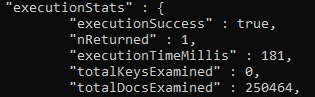
\includegraphics[width=0.9\linewidth]{img/UsernameNoIndex.png} 
		\caption{Results without index}
	\end{subfigure}
	\begin{subfigure}{0.5\textwidth}
		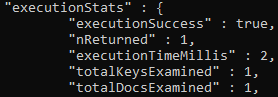
\includegraphics[width=0.9\linewidth]{img/UsernameIndex.png}
		\caption{Results with index}
	\end{subfigure}
\end{figure}

In the picture on the left is reported the output of the query when we do not use an index. Execution time is huge due to the very high number of docs examined. On the contrary, with an index, the same query need an execution time almost 100 times lower, and of course thanks to the index, DBMS only need to examinate one document. Moreover the unique property permits to eliminate the need of submitting query R1 at each registration.\\
Considering the very high speed-up ratio of the indexing and the high frequency of this kind of queries w.r.t. the write operations (as explained before), a UNIQUE INDEX on username has been created.

\subparagraph{Country}
As seen before, starting from the application queries we demonstrate the benefits of an index in the field \textit{country}.

\begin{center}
	\begin{tabular}{|c | c |} 
		\hline
		\textbf{Type} & \textbf{Query} \\ [0.5ex] 
		\hline
		\textbf{W1} & Insert the country data at registration timer \\ 
		\hline
		\textbf{W2} & Remove all the user’s data if a user is banned by an admin \\
		\hline
		\textbf{W3} & Changing of settings after a user changes residence’s country \\
		\hline
		\textbf{R1} & Rank all users by country \\
		\hline
		\textbf{R2} & Rank countries with the highest logins-per-day ratios \\
		\hline
	\end{tabular}
\end{center}

Let $x$ be the number of registrations-per-day (W1), w.r.t this number W2 and W3 are very rare operations. Indeed, even though we can expect mischievous behaviors from some user, the number of country changes will never be comparable with $x$.\\
On the other hand, in order to guarantee a read-your-own-write eventual consistency on ranking R1, this query is recomputed every time a user asks to see the ranking itself. Thus, since the gameplay is highly based on rankings, we can estimate that R1 frequency will be about $400x$.\\
Furthermore we have to consider R2. Despite the fact that this query is executed just once per day (so $frequency(R2) \ll x$), it is an asynchronous procedure sensitive to execution time since it needs to lock the entire collection, make it unavailable to users for a while.\\
As seen before, let us compare DBMS performances with and without a country index.

\begin{lstlisting}[language=python]
	> db.user.find({country:"Italy"}).explain("executionStats")
\end{lstlisting}

\begin{figure}[H]
	\begin{subfigure}{0.5\textwidth}
		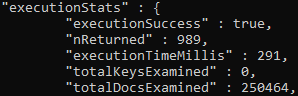
\includegraphics[width=0.9\linewidth]{img/CountryNoIndex.png} 
		\caption{Results without index}
	\end{subfigure}
	\begin{subfigure}{0.5\textwidth}
		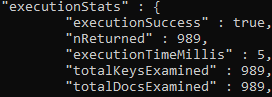
\includegraphics[width=0.9\linewidth]{img/CountryIndex.png}
		\caption{Results with index}
	\end{subfigure}
\end{figure}

Considering again about 250k users, without an index we need to scan the whole database, which means a medium-high execution time for each request.\\
On the contrary, we have a very high increase of performances introducing and index on country: execution time is about 58 times lower and the only documents examined are the ones that must be returned.\\
To summarize, considering the difference in frequency between reads and writes and the high decrease of execution time, an index on country has been introduced.

\subparagraph{Pokemon Name}

Queries on Pokémon’s name:

\begin{center}
	\begin{tabular}{|c | c |} 
		\hline
		\textbf{Type} & \textbf{Query} \\ [0.5ex] 
		\hline
		\textbf{W1} & Insert a new Pokémon into the Database \\ 
		\hline
		\textbf{W2} & Delete a Pokémon from the Database \\
		\hline
		\textbf{R1} & Search a Pokémon by name in the Pokédex \\
		\hline
		\textbf{R2} & Browse a Pokémon by name in Catch’Em’All in order to try to catch it \\
		\hline
		\textbf{R3} & Check name’s uniqueness of each Pokémon when added to the database \\
		\hline
	\end{tabular}
\end{center}

Again, W1 and W2 are rare and admin-related operations: this means that this queries will not require a frequent update of the index. On the contrary R1 and especially R2 are very frequent gameplay queries inside the application: we can estimate that R1+R2 frequency will be several orders of magnitude higher than W1+W2 one. \\
R3 instead is a query always required before W1, but it can be managed by DBMS adding a unique property to the index, thus reducing computational cost of the operation itself. \\
In terms of execution time, the final report is the following:  

\begin{lstlisting}[language=python]
	> db.user.pokemon({name: "pikachu"}).explain("executionStats")
\end{lstlisting}
\begin{figure}[H]
	\begin{subfigure}{0.5\textwidth}
		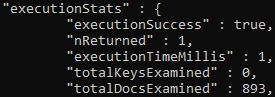
\includegraphics[width=0.9\linewidth]{img/PokemonNameNoIndex.png} 
		\caption{Results without index}
	\end{subfigure}
	\begin{subfigure}{0.5\textwidth}
		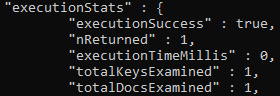
\includegraphics[width=0.9\linewidth]{img/PokemonNameIndex.png}
		\caption{Results with index}
	\end{subfigure}
\end{figure}


Even if we have little changes on execution time due to the limited number of \textbf{Pokémon}, we can see how the index permits to decrease very much the number of examined documents. \\
For the reasons explained before and because of the very high ratio between reads and writes, we consider this little improvement enough relevant for the application purposes. 

\subsection{Graph Database}
\subsubsection{Queries Handled}
\subsubsection{Entities handled}
\subsubsection{Graph structure}
\subsubsection{Indexes}


\subsection{Redundancies and consistency management}

\subsection{Database Properties}

\subsubsection{Availability}
\subsubsection{Replicas}
\subsubsection{Eventual Consistency}
\subsubsection{Sharding}
\subsubsection{Pros and Drawbacks}


\subsection{Client, Server and Daemon Thread}

\subsection{Technologies and Frameworks}

